% Сборка из tex/result: pdflatex -interaction=nonstopmode -halt-on-error edr_metric_corrections.tex (дважды).
\documentclass[11pt,a4paper]{article}
\usepackage[T2A]{fontenc}
\usepackage[utf8]{inputenc}
\usepackage[english,russian]{babel}
\usepackage[margin=21mm]{geometry}
\usepackage{amsmath,amssymb,amsthm,bm,booktabs,array,tabularx,graphicx,microtype}
\usepackage[hidelinks]{hyperref}
\usepackage{xurl}
\usepackage{enumitem}
\setlist{nosep,leftmargin=*}
\setlength{\parindent}{0pt}
\setlength{\parskip}{4pt}
\setlength{\emergencystretch}{3em}
\newcommand{\R}{\mathbb R}
\newcommand{\norm}[1]{\left\lVert#1\right\rVert}
\newcommand{\tr}{\operatorname{tr}}
\newcommand{\rank}{\operatorname{rank}}
\newcommand{\EDR}{\operatorname{EDR}}
\newcommand{\code}[1]{\nolinkurl{#1}}
\newtheorem{proposition}{Утверждение}
\newtheorem{theorem}{Теорема}
\newtheorem{remark}{Замечание}
\title{Коррекция моментного критерия ADP\\для восстановления EDR-подпространства}
\author{Систематизация идей \texttt{gpt\_ans.md}\\и воспроизводимые численные абляции}
\date{25 октября 2026 года}
\begin{document}
\maketitle
\begin{abstract}
Рассмотрены четыре различные задачи: нормировка точности локальных
моментов, устранение анизотропии измерительного оператора, балансировка
структурного спектра и ограничение ширины адаптивных ядер. Для каждой
поправки приведены формула, доказанное свойство и границы применимости.
Точное равенство нового функционала и квадрата EDR достигается при известных
градиентах полного структурного ранга. Для оценённых градиентов выведен
условный сертификат улучшения EDR. Практическая часть проверяет поправки
в существующем адаптивном ADP; её результаты отделены от теоретических
гарантий. Общедоступный алгоритм и его настройки не меняются.
\end{abstract}
\tableofcontents

\section{Постановка и обозначения}
Пусть наблюдаются
\[
 y_i=f(B_*^\top x_i)+\varepsilon_i,\qquad x_i\in\R^d,\quad
 B_*\in\R^{d\times m},\quad B_*^\top B_*=I_m,\quad m<d.
\]
Оценивается подпространство, поэтому базисы $B$ и $BQ$, $Q^\top Q=I_m$,
эквивалентны. Обозначим $P_B=BB^\top$, $P_*=B_*B_*^\top$ и
\begin{equation}\label{eq:edr}
 D(B)=\EDR^2(B,B_*)=\frac{\norm{(I-P_B)B_*}_F^2}{m}
 =\frac{\norm{P_B-P_*}_F^2}{2m}
 =\frac1m\sum_{r=1}^m\sin^2\theta_r.
\end{equation}
В таблицах эксперимента приводится $\EDR=\sqrt D$, а не $D$.

Для центра $a_j$ фиксированы веса $w_{ji}\ge0$, масса $N_j=\sum_iw_{ji}>0$,
нормированные веса $a_{ji}=w_{ji}/N_j$, средние
$\mu_j=\sum_i a_{ji}x_i$ и $\bar y_j=\sum_i a_{ji}y_i$. Пусть
\begin{align}
 C_j&=\sum_i a_{ji}(x_i-\mu_j)(x_i-\mu_j)^\top,&
 c_j&=\sum_i a_{ji}(x_i-\mu_j)(y_i-\bar y_j),\nonumber\\
 U_j&=\Phi_j C_j\in\R^{p\times d},&
 I_j&=\Phi_j c_j\in\R^p.\label{eq:moments}
\end{align}
Текущий внутренний Grassmann-солвер профилирует локальные коэффициенты:
\begin{equation}\label{eq:base}
 F(B)=\sum_j N_j\min_{g\in\R^m}\norm{I_j-U_jBg}^2,
 \qquad B^\top B=I_m.
\end{equation}
Моменты фиксированы внутри одного вызова, но пересчитываются между
внешними итерациями. В коде базис передаётся строками, то есть как $B^\top$.

\begin{center}\small
\begin{tabularx}{\linewidth}{@{}lXX@{}}
\toprule
Источник неравномерности & Поправка & Что она даёт \\
\midrule
Точность $I_j$ & $N_{{\rm eff},j}$ или GLS & Нормировку дисперсии \\
Геометрия $U_j$ & Отбеливание строк & Единичный спектр на наблюдаемом пространстве \\
Спектр градиентов & Полный проектор $P_V$ & Равный вес структурных направлений \\
Ширина ядра & Нижний порог $\Lambda$ & Контроль слабых направлений локализации \\
\bottomrule
\end{tabularx}
\end{center}
Поправки решают разные задачи. В частности, шумовая и геометрическая
метрики обычно не совпадают.

\section{Почему универсальная монотонность недостижима}
Желаемая импликация $F_{\rm new}(B_2)<F_{\rm new}(B_1)\Rightarrow
D(B_2)<D(B_1)$ не следует из наблюдений для всего неограниченного класса
гладких функций на конечной выборке.

\begin{proposition}[Неидентифицируемость на конечных данных]
Пусть проекции $B_s^\top x_i$, $i=1,\ldots,n$, попарно различны
для каждого из двух разных подпространств $s=0,1$. Любые значения $y_i$
можно представить одновременно как $f_s(B_s^\top x_i)$ с
$f_s\in C^\infty(\R^m)$.
\end{proposition}
\begin{proof}
Вокруг конечного числа различных проекций выбираются непересекающиеся
шары и гладкие функции с компактным носителем, равные единице в
соответствующих точках. Их линейная комбинация с коэффициентами $y_i$
интерполирует данные. Построение выполняется независимо для обоих $s$.
\end{proof}
Если функционал на таких данных строго предпочитает $B_1$, можно считать
истиной модель с $B_0$: ошибка в $B_0$ нулевая, а в $B_1$ положительная.
Следовательно, нет нетривиального универсального порядка кандидатов,
согласованного со всеми совместимыми истинами. Это утверждение не
отрицает идентифицируемость в ограниченном статистическом классе,
асимптотическую состоятельность или условные вероятностные гарантии.

\section{Точность локальных моментов: \texorpdfstring{$N_{\rm eff}$}{N-eff} и GLS}
\subsection{Эффективное число наблюдений}
Для взвешенного среднего дисперсия пропорциональна $\sum_i a_{ji}^2$,
поэтому
\begin{equation}\label{eq:neff}
 N_{{\rm eff},j}=\frac1{\sum_i a_{ji}^2}
 =\frac{(\sum_iw_{ji})^2}{\sum_iw_{ji}^2}.
\end{equation}
Замена внешней массы $N_j$ на $N_{{\rm eff},j}$ исправляет скалярный
масштаб, но не различие дисперсий и корреляцию компонент $I_j$.

\subsection{Полная ковариация внутри одного центра}
Предположим $\mathbb E[\varepsilon\mid X]=0$ и
$\operatorname{Cov}(\varepsilon\mid X)=\sigma^2 I_n$.
Веса и $\Phi_j$ фиксированы при условии $X$. Центрирование отклика
не создаёт дополнительного члена, поскольку
$\sum_i a_{ji}(x_i-\mu_j)=0$. Поэтому шум момента равен
\[
 \zeta_j=\sum_i a_{ji}\Phi_j(x_i-\mu_j)\varepsilon_i.
\]
Отсюда непосредственно
\begin{equation}\label{eq:covariance}
 \operatorname{Cov}(\zeta_j\mid X)=\sigma^2D_j,\qquad
 D_j=\sum_i a_{ji}^2\Phi_j(x_i-\mu_j)(x_i-\mu_j)^\top\Phi_j^\top.
\end{equation}
При $D_j\succ0$ естественен блочный критерий
\begin{equation}\label{eq:gls}
 F_{\rm GLS}(B)=\sum_j\min_g
 (I_j-U_jBg)^\top D_j^{-1}(I_j-U_jBg).
\end{equation}
\textbf{Внешнего множителя $N_j$ в этой формуле нет.}
Ковариация уже содержит квадраты нормированных весов.

\begin{theorem}[Нормированный шумовой вклад]
Если сигнальный момент точен, $I_j^{(0)}=U_jB_*g_j^*$,
а $\rank(D_j^{-1/2}U_jB_*)=m$, то
\[
 \mathbb E\!\left[\min_g\norm{D_j^{-1/2}(I_j-U_jB_*g)}^2\mid X\right]
 =\sigma^2(p-m).
\]
\end{theorem}
\begin{proof}
Пусть $A=D_j^{-1/2}U_jB_*$. После профилирования остаток равен
$(I-P_A)D_j^{-1/2}\zeta_j$. Его ожидаемый квадрат нормы равен
$\sigma^2\tr(I-P_A)=\sigma^2(p-m)$.
\end{proof}
Гауссовость не требуется. При ранге $D_j=r_j<p$ и использовании
псевдообратной аналогичная формула на образе $D_j$ имеет вид
$\sigma^2[r_j-\rank(D_j^{\dagger/2}U_jB_*)]$.

Ограничения результата: нелинейный моментный остаток не исчезает;
разные центры коррелированы через общие наблюдения; адаптивные веса,
полученные из тех же шумных откликов, не удовлетворяют условию
фиксированного дизайна. Поэтому \eqref{eq:gls} здесь является блочной
GLS-поправкой, а не полным совместным GLS для всех центров.

\section{Геометрия измерений: отбеливание строк}
Если $U_j$ имеет полный строчный ранг, положим
\begin{equation}\label{eq:row}
 W_j=(U_jU_j^\top)^{-1},\qquad
 F_{\rm row}(B)=\sum_jN_j\min_g\norm{W_j^{1/2}(I_j-U_jBg)}^2.
\end{equation}
Для любого $z\in\R^d$ справедливо
\begin{equation}\label{eq:rowprojector}
 \norm{W_j^{1/2}U_jz}^2
 =z^\top U_j^\top(U_jU_j^\top)^{-1}U_jz
 =\norm{P_{\operatorname{row}(U_j)}z}^2.
\end{equation}
Все ненулевые сингулярные значения $W_j^{1/2}U_j$ становятся единичными,
но ядро оператора остаётся прежним. Например, $U=[e_1,e_2]^\top$ в
$\R^3$, $m=1$, не различает прямые $\operatorname{span}(e_1)$ и
$\operatorname{span}(e_1+e_3)$ после профилирования масштаба $g$.

При $p=12,d=25$ размерность локального ядра $U_j$ не меньше $13$.
Совокупность центров может компенсировать локальные ядра, но одно
отбеливание этого не доказывает.

\textbf{Поправка к исходному тексту.} В реализации $N_{\rm loc}$ ---
целевая средняя масса ядра, а не число соседей. Если
$s_j=\#\{i:w_{ji}>0\}$, то
\[
 \rank(C_j)\le\min(d,s_j-1),\qquad
 \rank(U_j)\le\min(p,d,s_j-1).
\]
Подстановка $s_j=N_{\rm loc}=20$ без измерения носителя некорректна.

\section{Балансировка структурных направлений}
\subsection{Идеальные градиенты и спектральное искажение}
Пусть известны точные градиенты $v_j=B_*g_j^*$ и положительные веса
$\pi_j$. Определим
\[
 V=[\sqrt{\pi_1}v_1,\ldots,\sqrt{\pi_J}v_J],\qquad
 M=VV^\top=B_*GB_*^\top,\qquad
 G=\sum_j\pi_jg_j^*g_j^{*\top}.
\]
Для евклидовых градиентных невязок
\[
 F_0(B)=\sum_j\pi_j\min_g\norm{v_j-Bg}^2
 =\tr[(I-P_B)M]=\tr(TG),\quad
 T=B_*^\top(I-P_B)B_*.
\]
Так как $T\succeq0$ и $\tr T=mD(B)$, при
$0<\gamma=\lambda_{\min}(G)\le\lambda_{\max}(G)=\Gamma$ имеем
\begin{equation}\label{eq:bounds}
 \gamma mD(B)\le F_0(B)\le\Gamma mD(B).
\end{equation}
Оценка не задаёт монотонного порядка по $D$. К тому же $F_0$ ---
идеальный критерий известных градиентов, а не автоматически текущий
скетчированный критерий \eqref{eq:base}.

Скалярные веса сделали бы $G=cI_m$, если бы такое положительное
решение существовало. В общем случае его нет: для $g_1=(1,0)^\top$,
$g_2=(1,1)^\top$ внедиагональный элемент $G$ равен $\pi_2$,
и его зануление уничтожает второе направление.

\subsection{Полная матричная балансировка}
\begin{theorem}[Точная геометрическая цель]\label{thm:balance}
Если $v_j\in\operatorname{range}(B_*)$ и $\rank V=m$, то
\begin{equation}\label{eq:balance}
 P_V=V(V^\top V)^\dagger V^\top=P_*,\qquad
 F_{\rm bal}(B)=\tr[(I-P_B)P_V]=mD(B).
\end{equation}
\end{theorem}
\begin{proof}
Полнота ранга и включение пространств дают
$\operatorname{range}(V)=\operatorname{range}(B_*)$. Обе матрицы
$P_V$ и $P_*$ --- ортогональные проекторы на это пространство.
Остальное следует из \eqref{eq:edr}.
\end{proof}
Положительные собственные значения $M$ заменяются единицами.
Это выравнивает веса направлений, но не создаёт отсутствующее направление.
На практике проектор вычисляется по тонкому SVD $V$, без формирования
плотной псевдообратной размера $J\times J$.

\textbf{Недопустимая подстановка.} Если брать $v_j=B\widehat g_j(B)$
из текущего ограниченного решения, то при полном ранге $P_V=P_B$ и
$F_{\rm bal}(B)\equiv0$. Нужны градиенты, оценённые без ограничения
на проверяемый $B$.

Для оценённой матрицы $\widehat V$ берутся первые $m$ левых сингулярных
векторов $\widehat B$ и проектор $\widehat P=\widehat B\widehat B^\top$.
Определим
\begin{equation}\label{eq:surrogate}
 \widehat L(B)=m-\tr(B^\top\widehat PB),\qquad
 \operatorname{grad}\widehat L(B)=-2(I-P_B)\widehat PB.
\end{equation}
Минимизация одной этой цели возвращает $\operatorname{range}(\widehat B)$.
Следовательно, балансировка уже оценённой OPG-матрицы не улучшает её
собственные векторы: качество предварительного проектора надо измерять
отдельно. При шуме нельзя использовать полный проектор на все столбцы
$\widehat V$: он часто имеет ранг $d$ и даёт постоянное значение $d-m$.

\subsection{Контрпример: уменьшение цели при росте ошибки}
Пусть $d=4,m=2$, $B_*=[e_1,e_2]$ и
$M=100e_1e_1^\top+e_2e_2^\top$. Сравним
\[
 B_1=[\sqrt{0.96}e_1+0.2e_3,\ e_2],\qquad
 B_2=[e_1,\ \sqrt{0.2}e_2+\sqrt{0.8}e_4].
\]
\begin{center}
\begin{tabular}{@{}lrr@{}}
\toprule
Величина & $B_1$ & $B_2$ \\
\midrule
$F_0$ & $4$ & $0.8$ \\
$D=\EDR^2$ & $0.02$ & $0.40$ \\
$\EDR$ & $0.141421$ & $0.632456$ \\
$F_{\rm bal}$ & $0.04$ & $0.80$ \\
\bottomrule
\end{tabular}
\end{center}
Первоначальная цель предпочитает $B_2$, хотя $D$ увеличивается в $20$
раз, а $\EDR$ --- в $\sqrt{20}$ раз. В исходном Markdown эти две
ошибки местами названы одинаково; здесь различие сохранено.

\subsection{Итерация для точного проектора}
При известном $P_*$ можно положить
$B_{k+1}=\operatorname{orth}[(I+\tau P_*)B_k]$, $\tau>0$.
Если все начальные главные углы меньше $\pi/2$, подпространство
представляется графиком $K_0$ над истинным подпространством.
Умножение преобразует его в $K_{k+1}=K_k/(1+\tau)$. Поэтому
\begin{equation}\label{eq:iteration}
 D(B_k)=\frac1m\sum_{r=1}^m
 \frac{s_r^2(1+\tau)^{-2k}}{1+s_r^2(1+\tau)^{-2k}},\qquad
 s_r=\tan\theta_r(0),
\end{equation}
и $D(B_k)\le\norm{K_0}_F^2(1+\tau)^{-2k}/m$.
Итерация требует $O(dm^2+m^3)$ операций и $O(dm)$ памяти.
При угле $\pi/2$ эта гарантия неприменима. Для $\widehat P$ формула
описывает сходимость к оценённому, а не к истинному подпространству.

\section{Сертификат улучшения при оценённых градиентах}
\subsection{Детерминированная граница}
Предположим, что столбцы истинной $V$ лежат в $\operatorname{range}(B_*)$,
а для предварительной оценки установлено
\begin{equation}\label{eq:t}
 \norm{\widehat V-V}_2\le t.
\end{equation}
Пусть $\widehat B$ ортонормирован; определим
\begin{align*}
 \widehat M&=\widehat V\widehat V^\top,&
 \widehat\Lambda&=\widehat B^\top\widehat M\widehat B,&
 R&=\widehat M\widehat B-\widehat B\widehat\Lambda,\\
 q&=\lambda_{\min}(\widehat\Lambda)>0,&
 \delta&=2\norm{\widehat V}_2t+t^2.
\end{align*}
\begin{theorem}[Условный сертификат EDR]\label{thm:certificate}
В точной арифметике
\begin{equation}\label{eq:certificate}
 \EDR(\widehat B,B_*)\le e_{\rm cert}
 :=\min\left\{1,\frac{\delta+\norm R_F/\sqrt m}{q}\right\}.
\end{equation}
Для любых $B_1,B_2$ условие
\begin{equation}\label{eq:accept}
 \widehat L(B_1)-\widehat L(B_2)>2m e_{\rm cert}
\end{equation}
гарантирует строгое уменьшение $D$, а значит, и $\EDR$.
\end{theorem}
\begin{proof}
Из \eqref{eq:t} следует
$\norm{\widehat M-VV^\top}_2\le\delta$.
Поскольку $(I-P_*)VV^\top=0$, имеем
\[
 (I-P_*)\widehat B\widehat\Lambda
 =(I-P_*)(\widehat M-VV^\top)\widehat B-(I-P_*)R.
\]
После умножения на $\widehat\Lambda^{-1}$ получаем
$\norm{(I-P_*)\widehat B}_F\le(\sqrt m\,\delta+\norm R_F)/q$.
Деление на $\sqrt m$ даёт первую оценку; дополнительно $\EDR\le1$.
Ненулевые собственные значения $\widehat P-P_*$ образуют пары
$\pm\sin\theta_r$. Для любого проектора $P_B$ ранга $m$
\[
 |\tr[P_B(\widehat P-P_*)]|
 \le\sum_r\sin\theta_r
 \le m\EDR(\widehat B,B_*).
\]
Следовательно, равномерно по $B$
\begin{equation}\label{eq:uniform}
 |\widehat L(B)-mD(B)|\le m e_{\rm cert}.
\end{equation}
Вычитание двух таких неравенств даёт
$m[D(B_2)-D(B_1)]\le\widehat L(B_2)-\widehat L(B_1)+2me_{\rm cert}$,
что доказывает утверждение.
\end{proof}
Равномерность позволяет выбирать кандидатов адаптивно на тех же данных.
Однако предварительный проектор нельзя заново определять как
проектор на $B\widehat g_j(B)$ для каждого кандидата.
При $e_{\rm cert}\ge1/2$ принятие невозможно: левая часть
\eqref{eq:accept} не превосходит $m$.

\subsection{Получение границы \texorpdfstring{$t$}{t}}
Рассмотрим неограниченные локальные оценки $\widehat v_j=C_j^{-1}c_j$
с $C_j\succ0$ и весами, фиксированными по $X$. Пусть для регрессии
$g(x)=f(B_*^\top x)$ известна граница $\norm{\nabla^2g(x)}_2\le L$
на выпуклых областях, содержащих отрезки от центра до наблюдений.
Положим $v_j=\nabla g(a_j)$ и
$R_j=\max_{i:a_{ji}>0}\norm{x_i-a_j}$.
Разложение Тейлора даёт
\[
 c_j=C_jv_j+q_j+\zeta_j,\qquad \norm{q_j}\le LR_j^3.
\]
Действительно, остаток отклика не превосходит $LR_j^2/2$, а
$\norm{x_i-\mu_j}\le2R_j$. Для фиксированных $\pi_j>0$ определим
\begin{align}
 b_X&=L\left[\sum_j\pi_j
 \frac{R_j^6}{\lambda_{\min}(C_j)^2}\right]^{1/2},\nonumber\\
 s_X^2&=\sigma^2\sum_j\pi_j\sum_i a_{ji}^2
 \norm{C_j^{-1}(x_i-\mu_j)}^2.\label{eq:variance}
\end{align}
Для $\rho\in(0,1)$ имеем
\begin{equation}\label{eq:probability}
 \Pr\left\{\norm{\widehat V-V}_2
 \le b_X+s_X/\sqrt\rho\mid X\right\}\ge1-\rho.
\end{equation}
Норма матрицы смещения ограничивается через норму Фробениуса величиной
$b_X$. Для шумовой матрицы $Z$ выполнено
$\mathbb E[\norm Z_F^2\mid X]=s_X^2$ даже при корреляции столбцов;
неравенство Маркова и $\norm Z_2\le\norm Z_F$ завершают доказательство.

Здесь нужны достоверные верхние границы $L$ и $\sigma^2$.
Обычные точечные оценки не дают заявленной вероятности. При ridge
оценка $C_j^{-1}c_j$ меняется и требуется дополнительно ограничить
ridge-смещение. Для адаптивных по $Y$ весов нужен отдельный анализ
или независимая выборка для оценки статистик.

\textbf{Численная оговорка.} Малая невязка SVD учитывается членом $R$,
но не сертифицирует вычисление $\widehat V$, ортогональность или
округление скалярных границ. Если доказана ошибка построения матрицы
$t_{\rm round}$, в \eqref{eq:t} следует использовать $t+t_{\rm round}$.
Эксперимент ниже вычисляет диагностическую границу в float64;
это не интервальный сертификат машинной арифметики.

\subsection{Почему мягкий штраф не заменяет проверку шага}
Даже если $\widehat P=P_*$, у $F_\lambda=F_{\rm GLS}+\lambda\widehat L$
при конечном $\lambda$ не обязана быть стационарная точка в $B_*$.
Действительно, $\operatorname{grad}\widehat L(B_*)=0$, и если
$\operatorname{grad}F_{\rm GLS}(B_*)\ne0$, то
$\operatorname{grad}F_\lambda(B_*)\ne0$. Существует уменьшающий цель
шаг с положительной ошибкой вместо нулевой. Для строгой гарантии
нужна проверка \eqref{eq:accept}, а не произвольная сила штрафа.

\section{Спектральный порог анизотропии}
Для ортогонального тензора локализации
\[
 T_k^2=h_k^{-2}\{\alpha_k^2(I-P_{B_k})+B_k\Lambda_kB_k^\top\},
 \qquad \lambda_{\max}(\Lambda_k)=1,
\]
ширина вдоль собственного направления $\lambda_r$ равна
$h_k/\sqrt{\lambda_r}$. Слабое направление получает широкое окно.
Предлагается
\begin{equation}\label{eq:floor}
 \widetilde\Lambda_k=Q_k\operatorname{diag}\{\max(\lambda_{kr},\eta)\}Q_k^\top,
 \qquad 0<\eta\le1,
\end{equation}
и $\widetilde T_k^2$ с этой матрицей. При $0<\alpha_k\le1$
\begin{equation}\label{eq:condition}
 h_{kr}\le h_k/\sqrt\eta,\qquad
 \kappa_2(\widetilde T_k^2)\le\frac1{\min(\alpha_k^2,\eta)}.
\end{equation}
Если ядро компактно и $\theta_{\max}$ --- максимальный угол
между $B_k$ и $B_*$, то внутри его носителя
\begin{align}
 \norm{B_*^\top(x_i-a_j)}
 &\le h_k\left(\eta^{-1/2}+\frac{\sin\theta_{\max}}{\alpha_k}\right),\label{eq:radius}\\
 |r_{ji}|&\le\frac{Lh_k^2}{2}
 \left(\eta^{-1/2}+\frac{\sin\theta_{\max}}{\alpha_k}\right)^2,\nonumber\\
 \norm{c_j-C_j\nabla g(a_j)}
 &\le\frac{Lh_k^3}{\min(\alpha_k,\sqrt\eta)}
 \left(\eta^{-1/2}+\frac{\sin\theta_{\max}}{\alpha_k}\right)^2.\label{eq:bias}
\end{align}
Первое неравенство следует из разложения смещения на части вдоль
$B_k$ и ортогонально ему. Второе --- из Тейлора. Для третьего
используются $\norm{x_i-\mu_j}\le2h_k/\min(\alpha_k,\sqrt\eta)$
и нормировка весов.

При фиксированных $h_k,\alpha_k,\theta_{\max}$ увеличение $\eta$
уменьшает эту верхнюю границу смещения. В реальном ADP коэффициент
$\alpha_k$ подбирается заново по массе; меняются также дисперсия,
путь оптимизации и момент остановки. Поэтому \eqref{eq:bias}
не доказывает улучшение EDR полного адаптивного процесса.
При $\alpha_k=0$ приведённые границы с делением на $\alpha_k$
неприменимы.

\section{Привязка к текущему коду и практический протокол}
\subsection{Изолированная реализация}
Статистики строятся функцией \code{calculate_statistics}; внешний цикл
\code{fit_index} позволяет передать собственную функцию статистик.
Новые поправки размещены в \code{experiments/edr_metric_corrections.py}.
Солвер, генератор центров, ядро, правила отбора шага и публичные настройки
сохранены. Спектральный порог уже реализован в
\code{AdaptiveCentersConfig(lambda_floor=eta)} и применяется и в весах,
и при поиске следующего коэффициента анизотропии.

Поскольку адаптер солвера умножает невязку на $N_j$, в GLS ему передаются
\[
 \widetilde I_j=N_j^{-1/2}D_j^{-1/2}I_j,\qquad
 \widetilde U_j=N_j^{-1/2}D_j^{-1/2}U_j.
\]
Это реализует именно \eqref{eq:gls}. Для $N_{\rm eff}$ оба момента
умножаются на $\sqrt{N_{{\rm eff},j}/N_j}$, а для row whitening ---
на $(U_jU_j^\top)^{-1/2}$. Исходные массы сохранены в структурной
адаптации $\sum_jN_jg_jg_j^\top$: изменение критерия не смешивается
с дополнительным изменением этого правила.

В GLS и row whitening собственные значения ниже
$10^{-8}\lambda_{\max}$ поднимаются до этого уровня. Такие случаи
подсчитываются; точные теоремы об обратных относятся лишь к
нерегуляризованным положительно определённым матрицам.
Это ограничение существенно при вырожденных окнах.

В текущем алгоритме $N_{\rm lin}=50$ задаёт изотропную инициализацию
с ridge $10^{-8}$. Для диагностического сертификата отдельно
пересчитываются \emph{нерегуляризованные} локальные градиенты
на тех же фиксированных окнах; теорема для $C_j^{-1}c_j$ не
приписывается ridge-инициализатору.

\subsection{Замороженное сравнение}
Протокол записан до просмотра результатов в
\code{verification/edr-metric-20261025/PROTOCOL.md}.
Проверяются две функции при $m\in\{2,3,5\}$:
\[
 f_{\rm add}(z)=\sin z_1+\tfrac12z_2^2+
 0.35\sum_{r=3}^m\tanh z_r,\qquad
 f_{\rm quad}(z)=\sum_{r=1}^m z_r^2.
\]
Используются $n=5000,d=25$, независимый нормальный дизайн,
случайный ортонормированный истинный базис, стандартизация сигнала
и добавочный шум $0.3\varepsilon_i$, $\varepsilon_i\sim N(0,1)$.
Настройки: $J=300,p=12,N_{\rm loc}=20,N_{\rm lin}=50$,
CPU Grassmann, не более $20$ внутренних шагов за вызов;
текущие настройки солвера \code{relative_gn=True},
\code{quadratic_trials=3}, \code{constant_centers=True}.
Численный baseline определяется снимком исходников данного checkout,
а не результатами прежних версий алгоритма.

Разведочный этап: $3$ новых seed, $12$ вариантов --- baseline, GLS,
row, $N_{\rm eff}$, четыре порога $\eta\in\{0.01,0.05,0.1,0.2\}$
и GLS с каждым порогом. Выбирается один кандидат по геометрическому
отношению EDR на additive при $m=3,5$.

Проверка выбора: $10$ новых seed, кандидат против baseline.
Требуется снижение среднего EDR не менее $5\%$ отдельно на additive
$m=3$ и $m=5$, отрицательная верхняя граница $95\%$ парного интервала
изменения EDR на этих двух случаях и ухудшение не более $5\%$
в каждом из остальных случаев. Также требуются все полные пары
без ошибок и ортогональность с невязкой меньше $10^{-8}$.
Только после этого разрешены $20$ следующих seed для validation
с теми же условиями. Провал закрывает проверку без повторной настройки.

Bootstrap использует $10000$ повторов и пересэмплирует seed как
кластер: функции и размерности с общими $X$ не считаются независимыми
повторами. Время и RSS измеряются отдельно от качества; порога
ускорения в этом исследовании нет.

\subsection{Контроль корректности и интерпретации}
Проверены следующие свойства: ковариация $D_j$ совпадает с ковариацией
точного линейного оператора по отклику; профиль преобразованных моментов
совпадает с прямым плотным GLS/row/$N_{\rm eff}$; вырожденные ковариации
регуляризуются с явной диагностикой; сертификат ограничивает прямую
геометрическую ошибку; контрпример воспроизводит числа таблицы.
При аудите сохранённые EDR пересчитываются по проекторам независимо
от функции главных углов, использованной при обучении. Проверяются
хеши входов, снимков исходников, начальных базисов, весов и направлений
первого шага, полнота пар и повторный расчёт всех критериев допуска.

Истинный базис используется только для генерации и отчётных метрик.
Он не участвует в обучении, выборе внешнего шага или вычислении
предлагаемой моментной метрики. Выбор гипотезы по истине на
разведочных данных проверяется на новых seed.

\section{Результаты практической проверки}\label{sec:results}
\subsection{Разведочные абляции}
Разведочный этап служит только для выбора гипотезы; его улучшения не являются подтверждением на новых данных.
В таблице --- отношения средних EDR к baseline. Значение меньше единицы означает меньшую ошибку.
\begin{center}\small\setlength{\tabcolsep}{4pt}
\begin{tabular}{@{}lrrrrrr@{}}\toprule
 & \multicolumn{3}{c}{additive} & \multicolumn{3}{c}{quadratic}\\
Вариант & $m=2$ & $m=3$ & $m=5$ & $m=2$ & $m=3$ & $m=5$\\\midrule
gls & 0.877 & 1.054 & 0.956 & 0.790 & 0.800 & 0.710\\
row & 0.969 & 1.035 & 0.985 & 0.856 & 0.820 & 0.759\\
neff & 1.007 & 1.100 & 0.992 & 1.012 & 0.983 & 1.134\\
floor0.01 & 1.000 & 1.000 & 1.000 & 1.000 & 1.000 & 1.000\\
floor0.05 & 1.000 & 1.027 & 0.972 & 1.000 & 0.973 & 1.000\\
floor0.1 & 1.000 & 1.029 & 0.972 & 1.000 & 0.984 & 1.000\\
floor0.2 & 1.000 & 1.019 & 0.950 & 1.000 & 0.967 & 1.000\\
gls-floor0.01 & 0.877 & 0.995 & 0.958 & 0.790 & 0.800 & 0.710\\
gls-floor0.05 & 0.877 & 1.076 & 0.998 & 0.790 & 0.800 & 0.710\\
gls-floor0.1 & 0.877 & 1.092 & 0.963 & 0.790 & 0.800 & 0.710\\
gls-floor0.2 & 0.866 & 1.066 & 0.962 & 0.790 & 0.799 & 0.710\\
\bottomrule\end{tabular}\end{center}
Выбран кандидат \code{gls-floor0.01}; после выбора его настройки зафиксированы.
\subsection{Проверка выбранного кандидата на новых seed}
\textbf{selection: допуск не пройден.} 
Кластерный $95\%$ интервал среднего парного изменения EDR на additive $m=3,5$: $[-0.01733, 0.03669]$.
\begin{center}\small\setlength{\tabcolsep}{5pt}
\begin{tabular}{@{}lrrrrrr@{}}\toprule
Функция & $m$ & Начало & Baseline & Кандидат & Отношение & Победы\\\midrule
additive & 2 & 0.2448 & 0.0599 & 0.0533 & 0.890 & 8/10\\
additive & 3 & 0.5660 & 0.4811 & 0.4934 & 1.026 & 4/10\\
additive & 5 & 0.7133 & 0.6456 & 0.6496 & 1.006 & 5/10\\
quadratic & 2 & 0.2630 & 0.0649 & 0.0486 & 0.748 & 9/10\\
quadratic & 3 & 0.3683 & 0.0855 & 0.0557 & 0.651 & 10/10\\
quadratic & 5 & 0.3247 & 0.1158 & 0.0848 & 0.732 & 8/10\\
\bottomrule\end{tabular}\end{center}
Условия допуска: полные пары --- да; ортогональность --- да; снижение ошибки на основных случаях --- нет; отрицательный доверительный интервал --- нет; допустимая ошибка на остальных случаях --- да.
\textbf{Validation не запускалась}: заранее установленные условия selection не выполнены. Повторная настройка по этому этапу не проводилась.
\begin{center}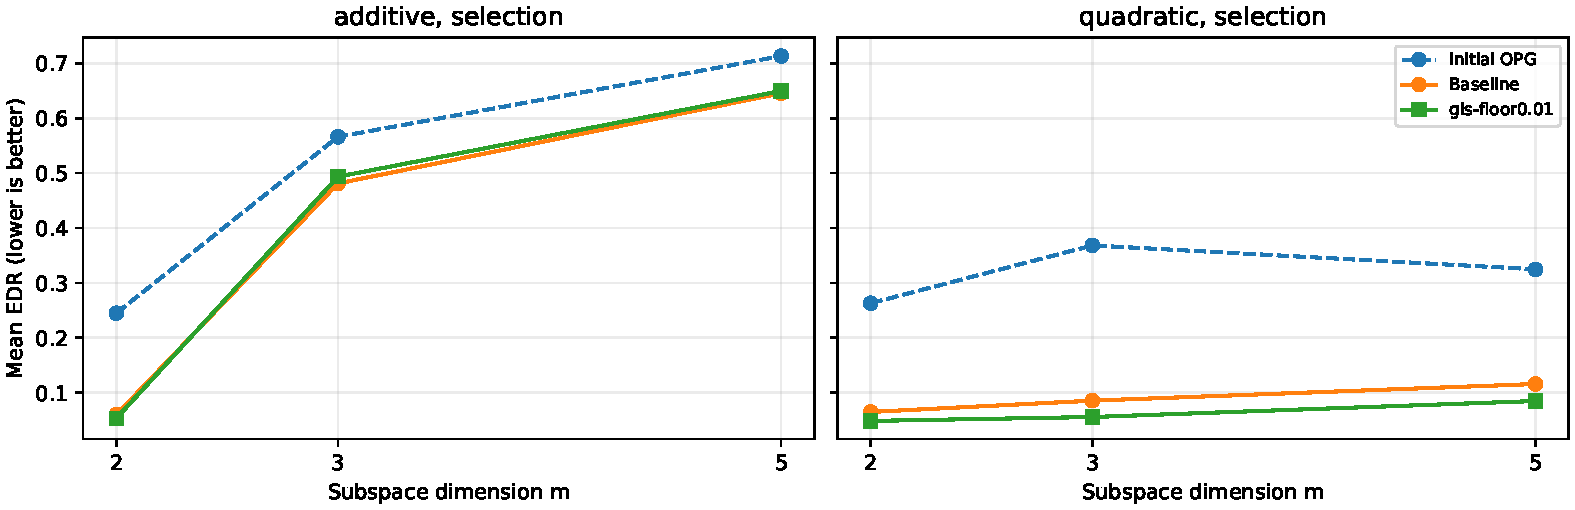
\includegraphics[width=\linewidth]{edr_metric_results_plot.pdf}\end{center}
\subsection{Время, память и диагностический сертификат}
\begin{center}\small\begin{tabular}{@{}lrr@{}}\toprule Величина & Baseline & Кандидат\\\midrule
Медиана fit time, с & 1.262 & 1.568\\
Медиана полного времени процесса, с & 1.651 & 1.896\\
Медиана peak RSS до диагностики, МиБ & 130.232 & 130.688\\
\bottomrule\end{tabular}\end{center}
Полное время включает запуск Python, загрузку данных и, у baseline, отдельную диагностическую процедуру (медиана 0.059 с). В fit time она не включена. Замеры выполнены при трёх конкурирующих процессах, BLAS по одному потоку; это не последовательный микробенчмарк.
\begin{center}\small\begin{tabular}{@{}lrr@{}}\toprule Диагностика внутренних вызовов & Baseline & Кандидат\\\midrule
Всего вызовов & 300 & 300\\
Сходимость по внутреннему критерию & 0 & 0\\
Остановка по max\_steps & 261 & 231\\
Вызовы с потерей локального ранга & 300 & 300\\
Применим гладкий критерий стационарности & 0 & 0\\
\bottomrule\end{tabular}\end{center}
Завершение fit без исключения означает получение конечного ортонормированного базиса, но не доказывает сходимость внутренних задач или достижение глобального минимума. Цели разных метрик имеют разный масштаб и по их значениям качество восстановления не сравнивается.
В 60/60 baseline-fit предварительная процедура встретила вырожденную $C_j$: условие теоремы $C_j\succ0$ не выполнено. Это возможно даже при средней массе 50: некоторые периферийные центры имеют слишком мало соседей. Ridge-инициализация остаётся определённой, но формулу для нерегуляризованных градиентов к ней применять нельзя. Сертифицированное принятие шага в таких fit не выполнялось.
Число центр--итераций с регуляризацией положительного спектра: 16043; с полностью нулевой ковариацией у кандидата: 1721. Нулевые информационные блоки дают нулевую невязку и сохраняются в трассе.
Аудит основного исследования: 336/336 успешных fit, геометрические ошибки и контрольные суммы сохранённых данных проверены повторно.
\subsection{Сохранённая первая попытка}
В \code{attempt1-zero-covariance} сохранён первоначальный запуск. Первый прототип ошибочно отклонял все нулевые ковариационные блоки; случай окна с единственным наблюдением воспроизведён отдельным тестом и исправлен. После исправления использованы новые диапазоны seed. Неудачи первой попытки не заменены успешными строками.
В первой попытке кандидат floor0.05 также не прошёл selection: $m=3$, отношение средних EDR 1.0349; $m=5$, отношение средних EDR 0.9931. Этот отрицательный результат сохраняет силу для той попытки.
\subsection{Вывод по эксперименту}
Выбранная поправка не прошла все заранее заданные условия. Локальные улучшения следует считать ограниченным эмпирическим эффектом; оснований менять стандартный алгоритм по этому эксперименту нет.


\section{Вычислительная цена и область применимости}
Для среднего носителя окна $s$, числа центров $J$ и числа направлений $p$
получение $D_j$ требует порядка $O(Js(pd+p^2))$ операций,
а его спектральные разложения --- $O(Jp^3)$.
Дополнительное хранение всех ковариаций равно $O(Jp^2)$;
при $J=300,p=12$ это $345600$ байт, примерно $0.33$ МиБ float64.
Это размер одного массива, а не измеренный RSS всего процесса.
В эксперименте блоки весов дополнительно буферизуются одинаково
для baseline и кандидатов, чтобы вычислить новые ковариации и хеши.

Row whitening требует $O(Jp^2d+Jp^3)$ операций. Нижний порог
диагонального $\Lambda$ требует $O(m)$ операций и $O(m)$ памяти;
его основной расход связан с изменившимся адаптивным процессом.
Тонкое SVD предварительной матрицы $d\times J$, $J\ge d$,
стоит $O(Jd^2)$ при хранении $O(Jd+d^2)$. Проверка $\widehat L(B)$
через базис $\widehat B$ стоит $O(dm^2)$.
Получение самих неограниченных градиентов через плотные локальные
ковариации может стоить $O(Jsd^2+Jd^3)$.

Теоретический результат относится к явно перечисленным предположениям.
Эксперимент проверяет конкретные функции, дизайн, шум и настройки;
он не превращает эмпирическую поправку адаптивного алгоритма
в универсальную гарантию восстановления. При слабом исходном проекторе
необходимо повышать точность локальных оценок; нормировка уже
потерянных градиентных направлений их не восстанавливает.

\appendix
\section{Воспроизведение и материалы}
Исходный материал: \code{tex/data/gpt_ans.md}; связанные постановки:
\code{tex/data/grassmann_solver_edr_problem.tex} и
\code{tex/data/multiindex.tex}. Систематизация исправляет обозначения,
выделяет условия доказательств и не переносит численные результаты
других checkout без повторного измерения.

Проверки и аудит из корня репозитория:
\begin{verbatim}
python3 -m pytest -q tests/test_edr_metric_corrections.py
python3 -m experiments.edr_metric_study audit
\end{verbatim}
Полный запуск на ещё не существующих выходных каталогах:
\begin{verbatim}
python3 -m experiments.edr_metric_study run
\end{verbatim}
Запуск отказывается перезаписывать замороженные этапы. Для новой
гипотезы требуются новый протокол, каталог и новые диапазоны seed.
Артефакты исследования находятся в
\code{verification/edr-metric-20261025/}: входы, полные результаты,
базисы и трассы, \code{sources.zip}, \code{manifest.json},
\code{decision.json}, \code{summary.csv} и \code{audit.json}.

Сборка документа дважды из каталога \code{tex/result}:
\begin{verbatim}
pdflatex -interaction=nonstopmode -halt-on-error \
  edr_metric_corrections.tex
\end{verbatim}
\end{document}
